\chapter{Echtzeitbetriebssysteme}
\section{Arten von Echtzeit}
\begin{itemize}
    \item Harte Echtzeit: Die Aufgabe muss zwingend vor der Deadline abgearbeitet sein
    \item Fest Echtzeit: Wenn die Information nach der Deadline kommen sind sie irrelevant
    \item Weiche Echtzeit: Die Aufgabe sollte meistens vor der Deadline abgearbeitet sein
\end{itemize}

\section{Aufgaben eines (Echtzeit-)Betriebssytems}
Standardaufgaben eines Betriebssytems:
\begin{itemize}
    \item Taskverwaltung
    \item Betriebsmittelverwaltung
    \item Interprozesskommunikation
    \item Synchronisationsaufgaben
    \item Schutzmaßnahmen
\end{itemize}
Ein Echtzeitbetriebssysteme (RTOS) muss zudem folgende Aufgaben erfüllen:
\begin{itemize}
    \item Rechtzeitigkeit
    \item Gleichzeitigkeit
    \item Verfügbarkeit
\end{itemize}

\section{Aufbau}
Ein (Echtzeit-)Betriebssytem ist normalerweise in einem Schichtenmodell aufgebaut.
\begin{figure}[H]
    \centering
    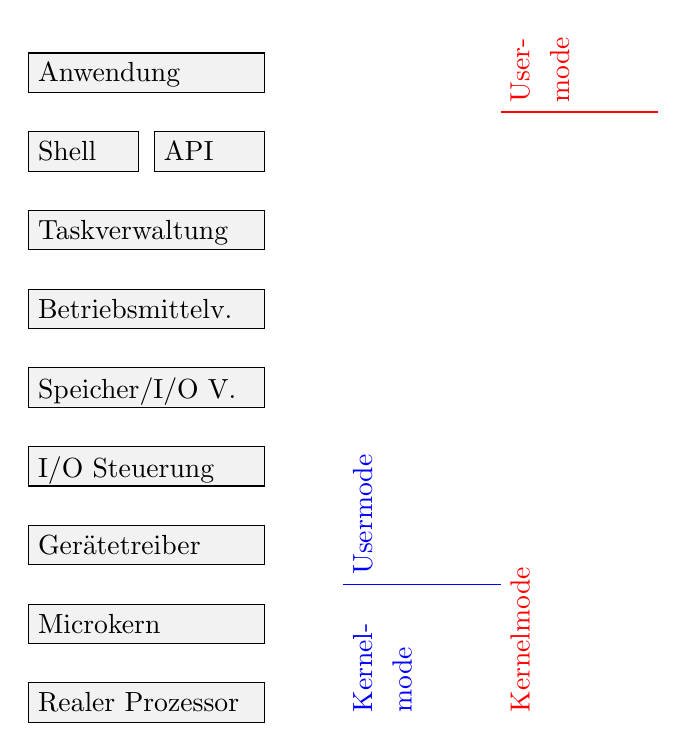
\begin{tikzpicture}
        \filldraw [draw=black,fill=gray!10] (3,0) rectangle (0,0.5) node [below right] {Realer Prozessor};
        \filldraw [draw=black,fill=gray!10] (3,1) rectangle (0,1.5) node [below right] {Microkern};
        \filldraw [draw=black,fill=gray!10] (3,2) rectangle (0,2.5) node [below right] {Gerätetreiber};
        \filldraw [draw=black,fill=gray!10] (3,3) rectangle (0,3.5) node [below right] {I/O Steuerung};
        \filldraw [draw=black,fill=gray!10] (3,4) rectangle (0,4.5) node [below right] {Speicher/I/O V.};
        \filldraw [draw=black,fill=gray!10] (3,5) rectangle (0,5.5) node [below right] {Betriebsmittelv.};
        \filldraw [draw=black,fill=gray!10] (3,6) rectangle (0,6.5) node [below right] {Taskverwaltung};
        \filldraw [draw=black,fill=gray!10] (3,7) rectangle (1.6,7.5) node [below right] {API};
        \filldraw [draw=black,fill=gray!10] (1.4,7) rectangle (0,7.5) node [below right] {Shell};
        \filldraw [draw=black,fill=gray!10] (3,8) rectangle (0,8.5) node [below right] {Anwendung};
        \draw [draw=blue] (4,1.75) -- (6,1.75);
        \node[below right,rotate=90, text=blue] at (4,0) (){Kernel-};
        \node[below right,rotate=90, text=blue] at (4.5,0) (){mode};
        \node[below right,rotate=90, text=blue] at (4,1.75) (){Usermode};
        \draw [draw=red] (6,7.75) -- (8,7.75);
        \node[below right,rotate=90, text=red] at (6,0) (){Kernelmode};
        \node[below right,rotate=90, text=red] at (6,7.75) (){User-};
        \node[below right,rotate=90, text=red] at (6.5,7.75) (){mode};
    \end{tikzpicture}
    \caption{Beispielhafter Aufbau eines Betriebssytems (Microkernel in \textcolor{blue}{blau}, Makrokernel/Monolithischer Kernel in \textcolor{red}{rot})}
\end{figure}

\section{Taskverwaltung}
Ein Task (\glqq{}Rechenprozess\grqq{}) ist ein ablaufendes Programm zusammen mit Variablen und Betriebsmitteln.
Tasks besitzen:
\begin{itemize}
    \item Aktionsfunktionen (\glqq{}Programm\grqq{})
    \item Zustandsvariablen (Speicher, Register, PC)
\end{itemize}
\todo{Grafik}
\subsection{Taskzustände}
\begin{figure}[H]
    \centering
    \includegraphics[width=\textwidth]{taskzustande.pdf}
    \caption{Zustandsmaschine der Taskübergänge}
\end{figure}
